\section{Results}\label{sec:results}

\begin{figure}[t]
\centering
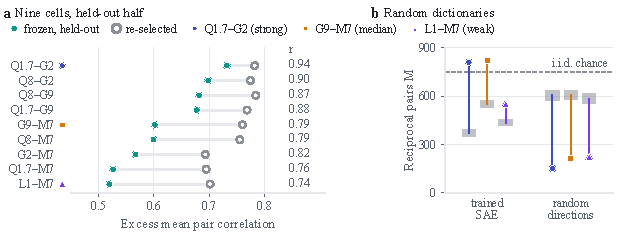
\includegraphics[width=\textwidth]{figures/results_20261010/main_results.pdf}
\caption{\textbf{The coactivation survives disjoint documents in all nine cells, and matched random directions do not reproduce it;} the control ladder is \Cref{fig:arc}, where on three representative cells every control has retention ratio $R\ge0.88$ against its reference arm, and length-decile nulls, run on six of the nine cells, leave at least $0.96$ of the excess (\Cref{app:lencov,app:ninecell}; all nine after submission). (a)~Pairs selected on $1{,}000$ C4 documents and frozen
(filled) vs.\ pairs re-selected on the evaluation half (open); $r$ is their ratio of excesses,
over two different pair sets (\Cref{prop:heldout}); every held-out $p=1/2001$. (b)~Reciprocal count $M$
(marker) against its own permutation null (grey, mean${\pm}2$\,SD) for trained SAEs and
size/sparsity-matched random directions; dashed: the i.i.d.\ chance level of
\Cref{prop:null}(a). Q/G/M/L $=$ Qwen3/Gemma-2/Mistral/Llama-3.2, number $=$ size (B). Drawn
by \texttt{code/figures/main\_results\_20261010.py} from \texttt{heldout\_*}, \texttt{c4\_*} and \texttt{rand\_c4\_*.json}.}
\label{fig:heldout-main}
\end{figure}

\subsection{Cross-model SAE feature matching}\label{sec:results:sae-matching}

We run the pipeline of \Cref{sec:method} on the pairs of \Cref{tab:sae-roster}, each model with
\emph{one} publicly released SAE (\texttt{sae-lens}, \citealp{bloom2024saelens}; Gemma Scope's is read one block
before its training hook, \Cref{app:gemmahook}) and mean-pooled features, so claims attach to
(model, SAE, read point, pooling) (\Cref{app:threats}).

\paragraph{Finding 1: the natural-text control decides which cells merit held-out testing.} On
the templated concept corpus every tested pair among Gemma-2, Mistral-7B and Pythia (models from $70$M to $9$B)
clears its reciprocal null (\Cref{tab:sae_matching}). The $2{,}000$-document C4 screen
\citep{raffel2020exploring} then separates candidates from a corpus artifact
(\Cref{tab:c4_counts}): Pythia-70M$\leftrightarrow$Mistral-7B, a cross-family cell strongly
significant on templates, \emph{falls to null on C4}; its sharing was template-tuned. The
modern ${\gtrsim}1$B pairs survive, and Qwen3-1.7B/8B (Qwen-Scope SAEs, \citealp{qwenscope2026};
manual adapter) share with both other families, as does Llama-3.2-1B
(\citealp{chanind2024llamasae}) against Mistral-7B (SAE: \citealp{engels2024mistralsae}): nine
cross-family cells across four families. In the non-pre-registered held-out follow-up, freezing
first-half pairs and scoring them on the second half confirms all nine at
$p=1/2001$, which clears Bonferroni over all $17$ C4 cells considered; held-out excess is
$74$--$94\%$ of the eval-half re-selected excess, a ratio over different pair sets, not
within-pair retention (\Cref{fig:heldout-main}a, \Cref{tab:c4_verdicts}). The templated corpus errs in both
directions: Qwen3-1.7B$\leftrightarrow$Gemma-2-2B is weak on templates ($z=3.59$, $p=1/201$) and strong on C4 ($z=42.7$), the
mirror image of the Pythia artifact, hence the natural-text headline.

\paragraph{What we do \emph{not} claim: no capability trend.} Against the fixed Mistral-7B
reference, $z$ rises with size across Pythia-70M, Llama-3.2-1B, Qwen3-1.7B, Gemma-2-2B and
Gemma-2-9B, which invites a reading as emergence with
capability and an SAE-level Platonic Representation Hypothesis \citep{huh2024platonic}. The axis
is confounded with the dictionary: these five cells pair Mistral's SAE with four other SAE suites, and
swapping only the Gemma-2-2B dictionary $16$k$\to$$65$k moves its cell from $z=22.1$ to $14.1$
with no change of model (\Cref{tab:c4_counts}). What survives is the per-cell verdict, which
needs no cross-cell comparison. GPT-2's four natural-text cells are underpowered (\Cref{app:threats}), so exactly one model is measured below null with power. On the
templated corpus both Gemma$\leftrightarrow$Mistral pairs are significant at all three depth bands
(\Cref{tab:sae_matching}); on C4 each model is read at one mid-layer hook.

\begin{table}[t]
\centering
\caption{\textbf{The control ladder: each rung is a way to explain the shared excess away, and on
three representative cells none does.} Values are
strong/median/weak (Qwen3-1.7B$\leftrightarrow$Gemma-\mbox{2-2B}, Gemma-2-9B$\leftrightarrow$Mistral-7B,
Llama-3.2-1B$\leftrightarrow$Mistral-7B). Ratios follow \eqref{eq:ratio}; lexical rows use the
governing $k{=}4096$. ``reg.'': rule and outcome branches registered before the receipt existed;
the held-out follow-up was not. Topic rows (revised after submission): the size-matched
calibration averages $20$ random partitions in the registered nine-cell run (\Cref{app:ninecell});
the submitted values used one partition (\Cref{tab:covctl}). Full tables: \Cref{tab:c4_verdicts,tab:rand_control,tab:covctl,tab:lextok,tab:lanpair,tab:proclex,tab:tokalign}.}
\label{tab:ladder}
\footnotesize
\setlength{\tabcolsep}{3pt}
\begin{tabular}{@{}lllr@{}}
\toprule
Rung & Statistic & strong/median/weak & $p$ \\
\midrule
C4 screen, $2{,}000$ docs & $M$ (null mean) & $811$ ($371.8$)/$819$ ($553.4$)/$551$ ($434.9$) & $1/201$ \\
Random directions (size, $L_0$ matched) & $M$ (null mean) & $152$ ($604.7$)/$212$ ($607.0$)/$223$ ($584.5$) & $1.0$ \\
Held-out frozen pairs, $1{,}000{+}1{,}000$ & $\Delta_E$ & $0.732$/$0.602$/$0.519$ & $1/2001$ \\
\quad ratio to re-selected pairs & $r$ & $0.936$/$0.791$/$0.739$ & --- \\
\midrule
Topic strata, $k{=}200$ & $R$ & $0.927$/$0.982$/$0.979$ & $1/2001$ \\
Topic strata, $k{=}500$ & $R$ & $0.986$/$1.033$/$0.974$ & $1/2001$ \\
Lexical residualization, mutual NN (reg.) & $R_{\text{lex}}$ & $0.933$/$0.942$/$0.918$ & $1/2001$ \\
\quad \citeauthor{lan2024universal} pairing rule (reg.) & $R_{\text{lex}}$ & $0.900$/$0.905$/$0.910$ & $1/2001$ \\
\quad Procrustes pairing, disjoint half (reg.) & $R_{\text{lex}}$ & $0.928$/$0.920$/$0.885$ & $1/2001$ \\
\midrule
Token-aligned, within-document order (reg.) & $S_1^{\text{clean}}$ (mean $r$) & $0.522$/$0.398$/$0.335$ & $1/2001$ \\
Current-word type, first design (leaky, audit) & $R_{\text{tok}}$ & $1.064$/$1.301$/$1.307$ & --- \\
Current-word type, leakage-clean (reg.) & $R_{\text{tok}}^{\text{clean}}$ & $0.925$/$0.986$/$0.977$ & $1/2001$ \\
\bottomrule
\end{tabular}
\end{table}

\paragraph{Random-dictionary control: informative, but its $z$ is not an effect size.}
\citet{korznikov2026sanity} report random directions rivalling trained SAE features. Replacing
each dictionary with size- and sparsity-matched random directions collapses the reciprocal count
while its permutation null \emph{rises} (\Cref{fig:heldout-main}b, \Cref{tab:ladder}), so $z$ lands
well below zero. We pre-registered two readings ($z\approx0$, or $z$ stays high) and the
outcome matched neither; as both the count and its null move, the negative $z$ is not an
effect size. Narrow claim: matched random projections do not reproduce reciprocal structure.

\paragraph{The strongest control: lexical residualization at interpretable corpus
size.} The remaining alternative is shared \emph{lexical} detectors. An earlier attempt on
$2{,}000$ documents could not adjudicate: its nuisance model explained almost nothing, and an
intervention that removes nothing excludes nothing. The rerun on $20{,}000$ C4 documents
(rule, thresholds and both outcome branches registered first) adds a hard adequacy gate against a
spectrum-matched shuffled design and scores the \emph{originally matched} pairs, frozen on the raw
features, rather than a rematch that could reconstitute the total from different pairs
(\Cref{app:threats}). The gate passes at every $k$, with nearly every feature beating the shuffled design, yet the
frozen pairs keep nearly all of their excess: residualization leaves $92$--$94\%$ of it
($R_{\text{lex}}=0.918$--$0.942$, \Cref{tab:ladder}). The gate's $\Delta R^2$ is a
margin over a shuffled design, \emph{not} variance captured. The nuisance model is a
stopword-stripped, SVD-truncated \emph{unigram} TF-IDF design (\Cref{tab:lextok}), and a lexical model
whose median per-feature $R^2$ tops out at $0.14$ captures almost none of what the two models
share. The shared-unigram hypothesis is therefore narrowed at the ranks tested, not closed.

\paragraph{The same control under other pairing rules.} The survival could belong to our
reciprocal criterion rather than to the shared structure. We therefore transplant the pairing
rule of \citet{lan2024universal} (each $A$ feature to its best $B$ feature, many-to-one) into the
identical pipeline, with five outcome branches registered pre-receipt and a reimplementation gate
read first: the $1$--$1$ fraction must fall inside the interval implied by their Tables~5--6, and
it does in all three cells. Their rule retains slightly less than ours in every cell, far above the
registered $0.30$ collapse bar (\Cref{tab:lanpair}, \Cref{app:lan}). An orthogonally
aligned pairing fitted on a disjoint half and scored on the other also survives
(\Cref{tab:proclex}). Survival is a property of the shared structure, not of one criterion.

\paragraph{Token-aligned: the registered follow-up.}\label{sec:results:tokalign}
Pooling makes the headline order-insensitive by construction, so we registered a token-aligned
test (three first-class branches, committed reader) before extracting per-token data. Per-token
activations on the same $20{,}000$ documents are aligned across tokenizers at whitespace-word
granularity (\Cref{app:tokalign}). $S_1$, the frozen pairs' within-document
centered correlation, is a quantity the pooled statistic cannot contain, and it beats a
within-document word-order-shuffle null in all three cells: token-aligned sharing is not
reducible to document means. $S_2$ conditions on the current word (type fixed effects against a
within-type derangement). The first design's $R_{\text{tok}}>1$ is reported but not
verdict-bearing, for selection leakage and non-commuting centerings (\Cref{app:tokalign}). The
registered leakage-clean rerun closes both routes by construction: disjoint selection/evaluation
halves, a universe re-screened on the selection half, a gated token stream with an aliasing
audit, joint fixed effects re-run under every null draw, and one common scored-pair mask (counts
in \Cref{tab:tokalign}; split/mask hashes in the \texttt{tokaclean20k\_*} receipts). Under it,
the shared occurrence-level variation survives joint document and normalized-current-word-type
fixed effects in all three cells (\Cref{tab:ladder}); the bigram arm is not selection-clean; no syntax or composition claim.

\paragraph{What do the matched features respond to?} Common lexical and topical document
properties (\Cref{app:matched-examples}); this does not establish semantic identity.

\paragraph{Finding 2: the loose criteria are confounded.} Greedy-max excess saturates for most modern and
GPT-2 pairings, including GPT-2$\leftrightarrow$Mistral-7B, which has
no reciprocal sharing above null; Hungarian assignment \citep{kuhn1955hungarian} ranks Gemma-2-2B$\leftrightarrow$GPT-2,
with few reciprocal matches, above every genuinely sharing Gemma$\leftrightarrow$Mistral pair. The
null does not remove this: optimal assignment over all screened features finds matches driven by
prompt-level covariates that pooling preserves (\Cref{tab:sae_matching,fig:greedy_scatter}).

\paragraph{Finding 3: the two ablation probes are inconclusive; within-model steering promotes overlapping tokens.} Single-feature
ablation is degeneration-prone (an apparently decisive Pythia$\leftrightarrow$Mistral result is
entirely a degeneration artifact), and group ablation is confounded by a prompt-fragility axis so
broad that even the within-family positive control fails (\Cref{tab:causal}, \Cref{app:causal}).
\emph{No cross-model causal intervention succeeded.} Within-model steering escapes both
confounds: steer each matched feature in its own model
($h \mathrel{+}= \beta s_f W_{\text{dec}}[f]$) and compare the identity of the top-$30$ promoted
token strings. Matched pairs share more strings than a derangement null ($1.26$ vs.\ $0.01$ of $30$ at $50$
pairs and $\beta{=}2$); the excess holds at $20$ pairs for $\beta\in\{2,8\}$ and replicates on
\mbox{Qwen3-1.7B}$\leftrightarrow$Gemma-2-2B (\Cref{app:causal}); the cricket-matched pair promotes
\emph{batsman/batting/cricket} in Gemma and \emph{batt/caught/declared} in Mistral. This is
activation-level evidence of similar functional roles at our read point, not cross-model intervention evidence.

\paragraph{Finding 4 (templated prompts only): cross-lingual sharing is weak within models and
language-conditional across them.} Matching a model's
English features against its own features on aligned zh/ja/ko prompts (\Cref{tab:xling_cells}),
within-model sharing is \emph{weak and graded}: significant for en--ja and en--zh in Gemma-2-9B,
marginal in Gemma-2-2B, \emph{null for en--ko in both}, while every matched-$N$ cross-model
English cell clears its null. Gemma~Scope \citep{lieberum2024gemmascope} is trained on an
English-dominant mix, so weak en--X may partly reflect dictionary coverage. Across models sharing
is \emph{language-conditional}: on Chinese the within-family Gemma pair shares strongly (shared
tokenizer, flagged) while Gemma-2-2B$\leftrightarrow$Mistral-7B, significant on English, collapses below
null (\Cref{tab:xling_cells}). These cells use the templated corpus, which Finding~1 shows can
mis-estimate sharing in both directions; they are descriptive.

\paragraph{Finding 5: zero-shot probe transfer is in-sample only.} A concept probe trained on
one model's matched features and applied unchanged to the other transfers perfectly on all three
modern pairs when the matching is fit on the same templated prompts (controls near chance), but
falls to chance when the matching is fit on independent C4 text, so the in-sample transfer does not by itself establish a shared interface
(\Cref{app:probe_transfer}).

\subsection{Cross-lingual signals under controls}\label{sec:results:secondary}\label{sec:results:construct-validity}\label{sec:results:probe-attribution}

\paragraph{The raw probe-attribution metric measures depth, not language.} All three controls converge (\Cref{tab:construct_validity}; trajectories in \Cref{app:raw-depth-detail}).
Layer-shuffle collapses the mean cross-lingual $r$ to about zero; the
mismatched-concept control keeps most of $r$, with Pythia-410M keeping all of it despite
being a predominantly English model; and the required class ordering is inverted. The raw
metric \textbf{fails construct validity}: it captures the shape of a model's per-layer
logit-lens trajectory, not cross-lingual transfer. The depth-corrected \emph{residual}
(real $-$ mismatched) appears to separate the classes at $n=20$ antonym pairs, with Pythia as the
sole English-only baseline.

\paragraph{Scaling the controls: the residual is not cross-lingually specific.}\label{sec:results:residual-scaleup}
With $206$ concept pairs, $17$ models and three further English-only families
(\Cref{tab:residual_scaleup}, \Cref{app:residual-scale-detail}), the gap disappears: Pythia was the
one English-only family with a near-zero residual, and GPT-2's residual is the largest of all
$17$ models. We report all three tests because they disagree. The bootstrap interval for the difference (multilingual minus English-only) lies entirely below
zero, nominally in the \emph{reverse} direction; the model-as-unit exact permutation test over all class
assignments is far from significant in the pre-registered direction and two-sided, and so is the
pair-level test (\Cref{tab:residual_scaleup}). \emph{No test detects a
multilingual advantage; the only interval that excludes zero (the bootstrap, whose unit, concept
pairs, is wrong for a claim about model classes) points the other way.} A lang-pair split refutes an
English-anchoring mechanism (the residual is larger on non-English pairs even for English-only
models), pointing to shared surface structure (CJK numerals, templated frames). No construct-valid
cross-lingual positive survives this battery.
